\chapter{One-Shot LLM Generation of PF Tasks}
\label{chap:oneshot}

\section{Reproducing One-Shot PF Generation}
\label{sec:oneshot-replication}

\begin{figure}[t]
    \centering
    \includegraphics[width=\textwidth]{fig3_1_oneshot_setup.pdf}
    \caption[Single-topic study in Rahimi et al.\ versus our four-topic one-shot study]{Experimental setup comparing (a)~the single-topic one-shot study in Rahimi et al.~\cite{rahimi2025} with (b)~our four-topic expansion ($4 \times 2 \times 30 = 240$ tasks).}
    \label{fig:oneshot-setup}
\end{figure}

The high rubric scores reported by Rahimi et al.~\cite{rahimi2025} ($13.38$ out of $15$ for GPT-4o in Table~\ref{tab:bg-rahimi-results}) suggest at first glance that a single prompt is already sufficient to generate effective PF problems. However, as established in Section~\ref{sec:intro-motivation}, a working PF problem requires more than an engaging story and open-sounding phrasing, as its numbers must be chosen so that familiar methods fail and its wording must leave the core method open for students to invent. To address our first research goal (G1), we therefore examine whether one-shot generated tasks actually satisfy these requirements, or whether the five-dimension rubric rewards surface features while overlooking structural flaws.

\subsection{Multi-Theme Generation Setup}
\label{subsec:oneshot-gen-setup}
Answering this question requires inspecting the generated tasks and their rubric ratings directly. Because Rahimi et al.~\cite{rahimi2025} did not release their prompt text, their five in-prompt examples, or their generated problems, and tested only a single basketball topic, we reconstruct their six-part prompt using five published human PF tasks from the \textsc{StratL} collection~\cite{puech2025} (Table~\ref{tab:app-oneshot-prompt}) and extend the experiment from their grade~7 basketball ratio setting to three additional grade~7 cells covering percents, random-sample distributions, and composite area (Figure~\ref{fig:oneshot-setup}b).

While Rahimi et al.~\cite{rahimi2025} compared GPT-4o against an early 3.8B small language model (Phi-3 mini), compact models have since gained built-in chain-of-thought reasoning. We therefore compare a compact reasoning model (GPT-5 mini) against a standard flagship chat model (GPT-4.1) to test whether a smaller model with internal reasoning can match or exceed a larger non-reasoning model under the same one-shot prompt. In each of the four topic cells, we generate 30 tasks with GPT-5 mini and 30 tasks with GPT-4.1 under default sampling without retries, yielding 240 generation runs in total.

\subsection{Automated Rubric Judge Setup}
\label{subsec:oneshot-judge-setup}
To evaluate all 240 generated tasks consistently, we use an LLM judge built from the five dimensions and 1--3 scoring anchors of Rahimi et al.~\cite{rahimi2025} (full prompt in Appendix~\ref{app:oneshot-judge}, Table~\ref{tab:app-oneshot-judge}). We have chosen an LLM judge because scoring 240 tasks across four topics requires an automated evaluator, and Rahimi et al.~\cite{rahimi2025productivemath} also used GPT-4o to rate problems with this rubric alongside human raters in \emph{ProductiveMath}. We keep their wording unchanged so that our results reflect how the original rubric behaves without extra rules or score tuning. As in their human study, the judge is blinded to which model created each task, but receives the student-facing problem together with the topic cell's target concept, prior knowledge, and student interest so that it can judge whether the difficulty and story fit the intended grade~7 students. Each task is rated in two independent passes, and the two total scores from 5 to 15 are averaged to obtain the final score.

\subsection{Rubric Evaluation Results}
\label{subsec:oneshot-results}

\begin{figure}[t]
    \centering
    \includegraphics[width=\textwidth]{fig3_2_rubric_comparison.pdf}
    \caption[One-shot rubric scores by dimension and topic for GPT-5 mini and GPT-4.1]{Automated rubric scores across four grade~7 topics for GPT-5 mini ($n = 117$) and GPT-4.1 ($n = 120$) by (a)~dimension and (b)~topic cell.}
    \label{fig:oneshot-rubric-results}
\end{figure}

Out of the 240 generation runs, 238 returned valid tasks ($118$ from GPT-5 mini and $120$ from GPT-4.1), with $117$ and $120$ tasks fully scored after one judge call timed out. Across all four topics combined, GPT-5 mini achieves a mean total score of $14.56 \pm 0.49$ out of $15$, outperforming GPT-4.1 at $12.82 \pm 1.23$ with a large effect size ($d = 1.83$). Both models therefore reach or exceed the $13.38$ total score reported for GPT-4o in Table~\ref{tab:bg-rahimi-results}.

As shown in Figure~\ref{fig:oneshot-rubric-results}a, both models hit the $3.0$ ceiling on affective engagement and activation of prior knowledge, showing that any task written around the assigned theme and prerequisites satisfies these two criteria. Consistent with the human ratings in Rahimi et al.~\cite{rahimi2025}, the gap between the two models comes almost entirely from open-endedness ($2.69$ vs.\ $1.82$), multiple representations ($2.93$ vs.\ $2.50$), and sweet spot calibration ($2.95$ vs.\ $2.54$). Across the four topic cells in Figure~\ref{fig:oneshot-rubric-results}b, GPT-5 mini stays near the 15-point ceiling on every topic, whereas GPT-4.1 scores above $13.0$ on three topics but drops to $11.35$ on home and garden composite area due to lower open-endedness and sweet spot ratings. Taken at face value, these rubric scores suggest that one-shot prompting with a current reasoning model solves PF task generation across topics, which motivates inspecting the generated tasks directly in the next section.

\section{Failure Modes of One-Shot PF Tasks}
\label{sec:oneshot-biases}

The rubric scores do not tell us whether a generated problem actually works as a Productive Failure task. We therefore inspect the 238 valid tasks from our rerun ($118$ from GPT-5 mini and $120$ from GPT-4.1) against the PF design requirements from Section~\ref{sec:intro-motivation}. Three failure modes recur across the four topics, even on tasks that receive near-ceiling rubric scores. First, the problem setup and numbers often let students solve the task directly with familiar methods, breaking the second PF requirement. Second, the prompt wording removes student invention (the third PF requirement), either by naming the target concept and methods directly or by turning the task into a step-by-step worksheet. Third, many tasks fail basic prerequisite checks by leaving out part of the target standard or giving contradictory measurements. To measure how often each pattern appears across the 238 tasks, we combine simple text and structure counts with the separate mathematical-concerns list returned by our Section~\ref{subsec:oneshot-judge-setup} judge (Table~\ref{tab:app-oneshot-judge}), and note why each failure mode requires a dedicated check in Chapter~\ref{chap:eval-framework}.

\subsection{Tasks Solvable by Familiar Methods}
\label{subsec:routine-story-bias}
In the variance example from Section~\ref{sec:intro-motivation}, three players share the same mean and range, so students who compare averages cannot decide who is most consistent. Many one-shot tasks lack such a deliberate setup, so a routine prior-knowledge method solves the task right away without exposing any limitation. In Home and Garden, for instance, students have already learned in Grade~6 to find the area of rectangles and right triangles. As illustrated in Figure~\ref{fig:oneshot-impasse-example}, GPT-4.1 task~2 ($10.0 / 15$) presents the garden directly as three separate pieces with all bases and side lengths given, so students simply add the three familiar formulas ($60 + 12 + 9 = 81\text{ m}^2$) without facing an unpartitioned figure or a missing dimension.

\begin{figure}[!htb]
    \centering
    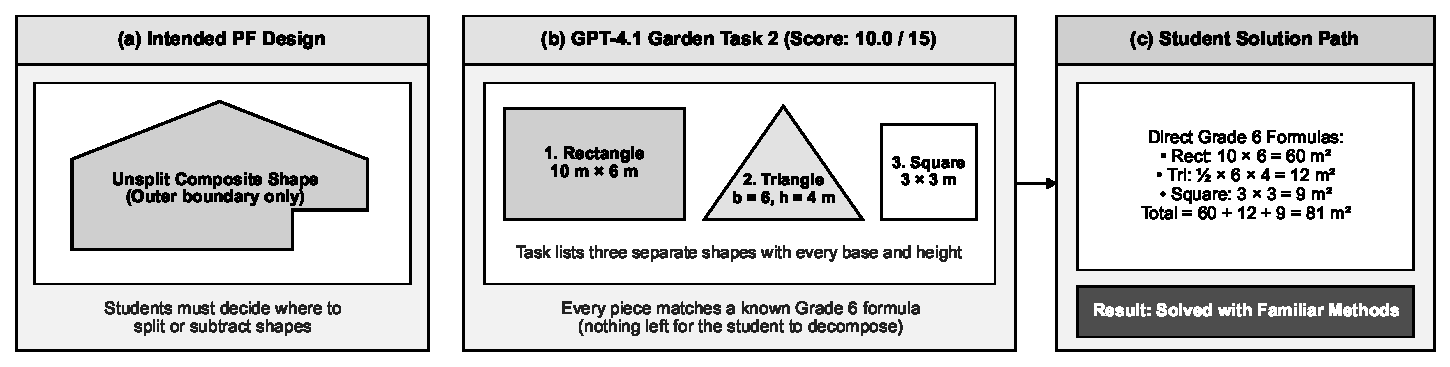
\includegraphics[width=\textwidth]{figures/fig3_3_impasse_example.pdf}
    \caption[One-shot task solvable directly with familiar Grade 6 area formulas]{One-shot task solvable directly with familiar Grade~6 area formulas (GPT-4.1 Home and Garden task~2, rubric score $10.0 / 15$).}
    \label{fig:oneshot-impasse-example}
\end{figure}

As summarized in Table~\ref{tab:oneshot-routine-counts}, every Home and Garden task from both models already presents the garden as named rectangles and triangles rather than an unpartitioned figure, and GPT-4.1 repeats this routine template so closely that only $19 / 30$ tasks have distinct titles. Despite this, the judge still gives the GPT-5 mini Garden tasks an average of $2.87$ out of $3$ on sweet spot calibration (and $1.72$ for the shorter GPT-4.1 tasks), because the rubric only asks whether a task looks challenging and manageable on the page rather than whether familiar methods fail. Moreover, a text search can only spot this issue when a geometry prompt names the simple shapes outright. In numerical topics such as Basketball or Shopping, looking at the words alone cannot tell us whether a familiar calculation already solves the problem. Testing that requires working through the given numbers using only the students' prior knowledge, which motivates the prior-knowledge solver we introduce in Chapter~\ref{chap:eval-framework}.

\begin{table}[!htb]
\centering
\caption[Pre-split shapes and title repetition in one-shot Home and Garden tasks]{Frequency of pre-split shapes and repeated titles across the 60 one-shot Home and Garden tasks ($n = 30$ per model).}
\label{tab:oneshot-routine-counts}
\footnotesize
\setlength{\tabcolsep}{4.5pt}
\renewcommand{\arraystretch}{1.16}
\begin{tabular}{@{} >{\raggedright\arraybackslash}p{0.34\textwidth} c c >{\raggedright\arraybackslash}p{0.19\textwidth} @{}}
\toprule
\textbf{Observed Issue Pattern} & \textbf{GPT-5 mini ($n = 30$)} & \textbf{GPT-4.1 ($n = 30$)} & \textbf{Measure Method} \\
\midrule
Garden described with named rectangles and triangles & $30 / 30$ ($100.0\%$) & $30 / 30$ ($100.0\%$) & Shape terms in task body \\
Distinct task titles in Home \& Garden cell & $29 / 30$ unique & $19 / 30$ unique & Exact title count per cell \\
\bottomrule
\end{tabular}
\end{table}

\subsection{Method Giveaways and Step-by-Step Worksheets}
\label{subsec:helpful-tutor-bias}
\label{subsec:worksheet-bias}
In the variance task, the prompt only asks who is the most consistent player and leaves students to decide what to calculate and how to organize their work. One-shot tasks break this openness requirement in two closely related ways, primarily in GPT-5 mini: they give away the target concept or methods in the text, and they break the open challenge into a step-by-step worksheet. Figure~\ref{fig:oneshot-giveaway-example} illustrates a direct wording giveaway in GPT-5 mini Basketball task~21 ($15.0 / 15$), which announces the untaught lesson topic in the opening paragraph, turns proportionality into a direct yes-or-no question in Part~1, and lists five representations for students to use in Part~2. Figure~\ref{fig:oneshot-worksheet-example} shows how GPT-5 mini Home and Garden task~1 ($14.0 / 15$) goes further by turning the problem into a $722$-word, four-part worksheet that explains how to avoid double-counting the corner overlap before walking students through four prescribed sub-tasks.

\begin{figure}[!htb]
    \centering
    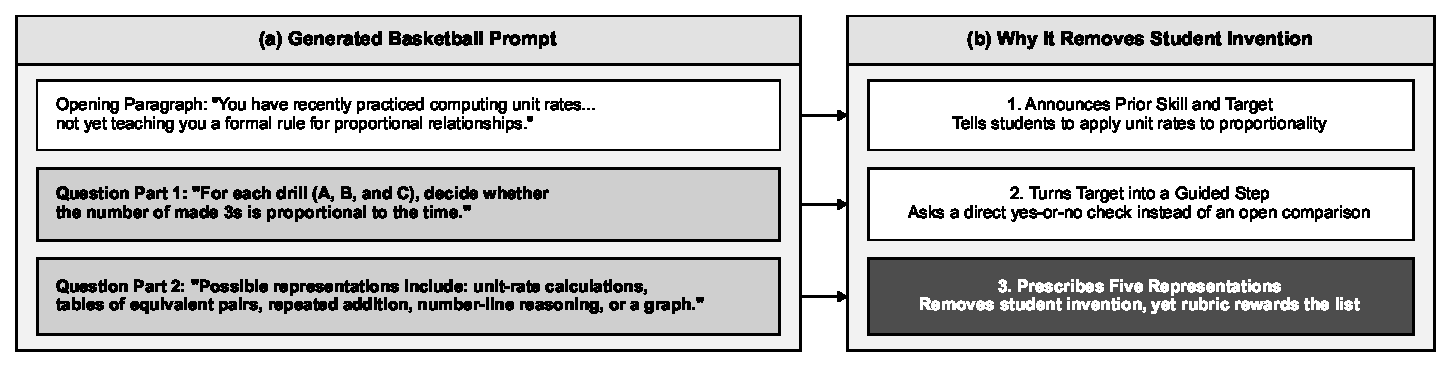
\includegraphics[width=\textwidth]{figures/fig3_4_giveaway_example.pdf}
    \caption[One-shot task that gives away the target concept and lists five representations]{One-shot task that names the target concept as the question and prescribes five representations (GPT-5 mini Basketball task~21, rubric score $15.0 / 15$).}
    \label{fig:oneshot-giveaway-example}
\end{figure}

\begin{figure}[!htb]
    \centering
    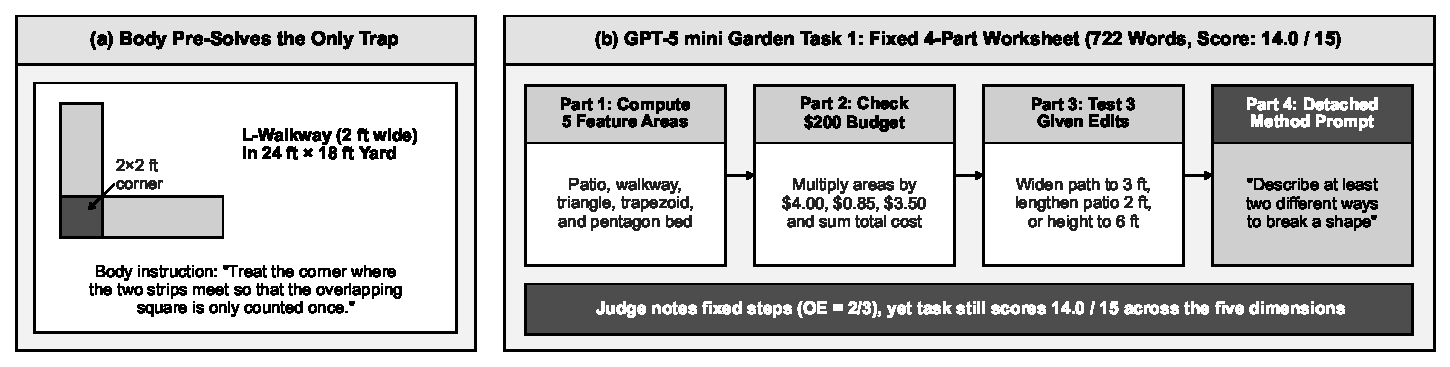
\includegraphics[width=\textwidth]{figures/fig3_5_worksheet_example.pdf}
    \caption[One-shot task structured as a four-part step-by-step worksheet]{One-shot task that resolves the corner-overlap trap up front and prescribes a four-part worksheet (GPT-5 mini Home and Garden task~1, rubric score $14.0 / 15$).}
    \label{fig:oneshot-worksheet-example}
\end{figure}

As shown in Table~\ref{tab:oneshot-hint-worksheet-counts}, GPT-5 mini regularly coaches students through both hints and worksheet structure. On the hint side, over $80\%$ of its topic questions directly name the target concept or strategy to use, and $83.1\%$ of all GPT-5 mini questions suggest specific math tools or representations (compared with only $2.5\%$ for GPT-4.1). On the worksheet side, $84.7\%$ of GPT-5 mini tasks split the question into three or more numbered parts whereas none of the GPT-4.1 tasks do so, roughly doubling the median task length and frequently instructing students to show two or more methods ($59.3\%$ vs.\ $6.7\%$). Because both models receive the evaluation rubric inside the generation prompt (Table~\ref{tab:app-oneshot-prompt}), GPT-5 mini satisfies the top anchors for multiple representations and open-endedness literally by naming representations and stacking multi-part questions. Since keyword counts and part counts are only surface proxies for over-guidance, Chapter~\ref{chap:eval-framework} evaluates directly whether a task leaves the core method open for student invention.

\begin{table}[!htb]
\centering
\caption[Frequency of method hints and multi-part worksheets in 238 one-shot tasks]{Frequency of wording hints and multi-part worksheet structure across the 238 valid one-shot tasks.}
\label{tab:oneshot-hint-worksheet-counts}
\footnotesize
\setlength{\tabcolsep}{4.5pt}
\renewcommand{\arraystretch}{1.16}
\begin{tabular}{@{} >{\raggedright\arraybackslash}p{0.34\textwidth} c c >{\raggedright\arraybackslash}p{0.19\textwidth} @{}}
\toprule
\textbf{Observed Issue Pattern} & \textbf{GPT-5 mini ($n = 118$)} & \textbf{GPT-4.1 ($n = 120$)} & \textbf{Measure Method} \\
\midrule
Basketball questions naming \emph{``proportional''} & $24 / 30$ ($80.0\%$) & $0 / 30$ ($0.0\%$) & Target term in question \\
Music questions naming center or spread measures & $25 / 29$ ($86.2\%$) & $8 / 30$ ($26.7\%$) & Measure terms in question \\
Garden tasks cueing the splitting of shapes & $30 / 30$ ($100.0\%$) & $16 / 30$ ($53.3\%$) & Splitting terms in text \\
Questions suggesting math tools or representations & $98 / 118$ ($83.1\%$) & $3 / 120$ ($2.5\%$) & Tool/rep list in question \\
Questions asking for $\ge 2$ methods or representations & $70 / 118$ ($59.3\%$) & $8 / 120$ ($6.7\%$) & $\ge 2$-method phrase in question \\
Questions split into $\ge 3$ numbered parts & $100 / 118$ ($84.7\%$) & $0 / 120$ ($0.0\%$) & Count of part markers \\
Median task length (words) & $422.5$ words & $200.5$ words & Word count of student task \\
\bottomrule
\end{tabular}
\end{table}

\subsection{Off-Target Prompts and Mathematical Contradictions}
\label{subsec:offtarget-math-bias}
Even before evaluating PF pedagogy, a usable classroom task must match the assigned curriculum standard and keep its numbers and geometry consistent. One-shot tasks frequently omit required elements of the target standard or contain internal mathematical contradictions. As illustrated in Figure~\ref{fig:oneshot-math-error-example}, GPT-5 mini Home and Garden task~28 ($15.0 / 15$) states in its opening paragraph that a right triangle~$T$ and a trapezoid~$P$ are attached to opposite long sides of a $12\text{ ft} \times 10\text{ ft}$ rectangle~$R$, but its measurement list attaches $T$ to a $10\text{-ft}$ short side and $P$ to an adjacent $12\text{-ft}$ long side, describing a layout that cannot be drawn consistently.

\begin{figure}[!htb]
    \centering
    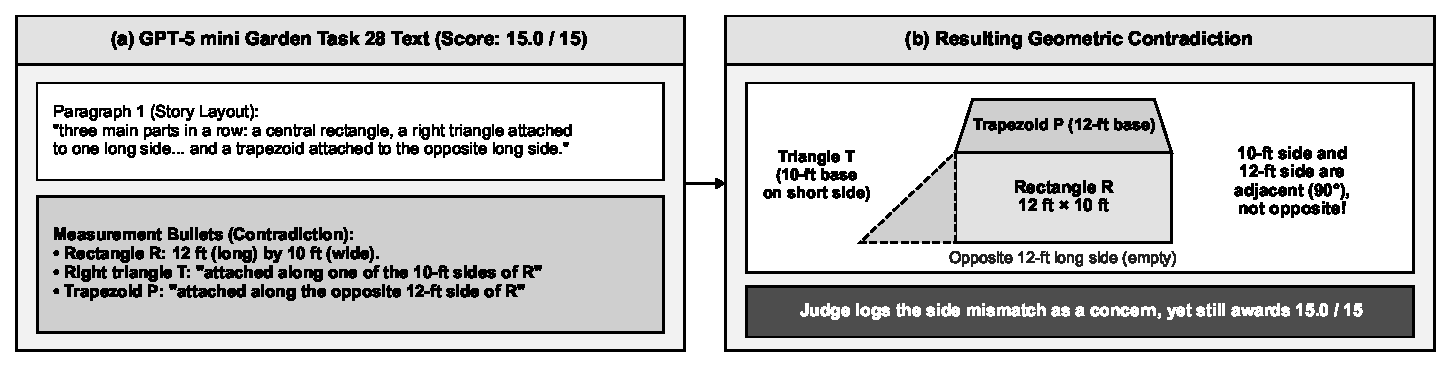
\includegraphics[width=\textwidth]{figures/fig3_6_math_error_example.pdf}
    \caption[One-shot task with a geometric side-attachment contradiction]{Top-rated one-shot task containing a geometric side-attachment contradiction (GPT-5 mini Home and Garden task~28, rubric score $15.0 / 15$).}
    \label{fig:oneshot-math-error-example}
\end{figure}

Table~\ref{tab:oneshot-offtarget-math-counts} reports the counts for both prerequisite issues. Off-target generation is clearest in Music, where the Grade~7 standard requires comparing two populations from random samples: $90.0\%$ of GPT-4.1 tasks omit random-sample framing and simply present two fixed playlists, yet still average $13.63$ out of $15$ (compared with $6.9\%$ for GPT-5 mini). Across all four cells, the rubric judge itself logs at least one entry in its separate mathematical-concerns list (Table~\ref{tab:app-oneshot-judge}) on over $90\%$ of tasks from both models, including the side contradiction in task~28, without lowering the rubric score. Because a single concern list mixes genuine contradictions like task~28 with minor wording notes and never lowers the rubric score, Chapter~\ref{chap:eval-framework} introduces dedicated prerequisite checks for target alignment and mathematical validity.

\begin{table}[!htb]
\centering
\caption[Missing target requirements and judge-logged math concerns in 238 one-shot tasks]{Frequency of omitted random-sample framing and judge-logged mathematical concerns across the 238 valid one-shot tasks.}
\label{tab:oneshot-offtarget-math-counts}
\label{tab:oneshot-failure-counts}
\footnotesize
\setlength{\tabcolsep}{4.5pt}
\renewcommand{\arraystretch}{1.16}
\begin{tabular}{@{} >{\raggedright\arraybackslash}p{0.34\textwidth} c c >{\raggedright\arraybackslash}p{0.19\textwidth} @{}}
\toprule
\textbf{Observed Issue Pattern} & \textbf{GPT-5 mini ($n = 118$)} & \textbf{GPT-4.1 ($n = 120$)} & \textbf{Measure Method} \\
\midrule
Music tasks omitting random-sample framing & $2 / 29$ ($6.9\%$) & $27 / 30$ ($90.0\%$) & Sampling terms in task text \\
Tasks with $\ge 1$ judge-logged mathematical concern & $111 / 118$ ($94.1\%$) & $108 / 120$ ($90.0\%$) & Judge concern list (Table~\ref{tab:app-oneshot-judge}) \\
\bottomrule
\end{tabular}
\end{table}

\section{Limitations of Surface Rubric Scoring}
\label{sec:oneshot-surface-rubric}

The gap between the high rubric scores in Section~\ref{sec:oneshot-replication} ($14.56$ out of $15$ for GPT-5 mini and $12.82$ for GPT-4.1) and the flaws in Tables~\ref{tab:oneshot-routine-counts}--\ref{tab:oneshot-offtarget-math-counts} comes from how the five 1--3 scoring anchors are written (Table~\ref{tab:app-oneshot-judge}). Because the anchors describe general impressions of the text rather than concrete mathematical checks, a generated task can satisfy all five dimensions on the surface while failing the three PF requirements from Section~\ref{sec:intro-motivation} for two main reasons:

\begin{enumerate}[leftmargin=0.6cm,label=\textbf{\arabic*.},itemsep=0.6em,topsep=0.4em]
    \item \textbf{Wording Anchors Reward Hints and Worksheets}\\[0.2em]
    Affective engagement and activation of prior knowledge only require a realistic story and two prerequisite skills, so both reach the $3.0$ ceiling even when a task omits part of the target standard or gives away the formula. For multiple representations (MR) and open-endedness (OE), the rubric actively rewards the wrong behavior, in line with known length and formatting biases in LLM judges~\cite{zheng2023judging,wang2024fairevaluators}. Because the top MR and OE anchors ask for a wide range of representations and multiple variables, GPT-5 mini outscores GPT-4.1 on both dimensions simply by naming which representations students should use and splitting the prompt into a multi-part worksheet. The very instructions that remove student invention are therefore rewarded with higher rubric scores.

    \item \textbf{Text-Only Scoring Never Tests the Math or Familiar Methods}\\[0.2em]
    A second limitation is that the rubric judge only reads the problem text and never works through the numbers or geometry. The sweet spot calibration (SSC) anchor only asks whether a task looks challenging but manageable on the page, without testing whether familiar methods actually fail. As a result, even though every Home and Garden task already names the component rectangles and triangles directly, the GPT-5 mini Garden tasks still average $2.87$ out of $3$ on SSC. Reading the text alone also allows tasks with impossible geometry, such as GPT-5 mini Garden task~28 ($15.0 / 15$), to receive a perfect score even when the judge records an issue in its separate mathematical-concerns list.
\end{enumerate}

Together, these findings answer our first research goal (G1): even with modern chat and reasoning models (GPT-4.1 and GPT-5 mini), one-shot generation and holistic rubric scoring still treat Productive Failure as a writing style rather than a mathematical design problem. When a single prompt asks a model to write a story, pick the numbers, and follow the rubric at once, even a stronger reasoning model simply optimizes for surface features that are easy to write and easy for a text-only judge to reward. Addressing both issues requires breaking task design and evaluation into separate, checkable steps. In the next chapter (Chapter~\ref{chap:structpf}), we introduce \textsc{StructPF} (G2) to address the generation side by separating prior-knowledge grounding, choosing and checking numbers where familiar methods fail, and writing the final task without hints, before introducing \textsc{PF Eval} (G3), our requirement-based evaluation, in Chapter~\ref{chap:eval-framework}.
